% Preambel mit Einstellungen importieren
% Document type and used packages
\documentclass[openany,
%    open=right, % Kapitel darf nur auf rechten Seite beginnen
    paper=A4,               % DIN-A4-Papier
    a4paper,                % DIN-A4-Papier
    12pt,                   % Schriftgöße
    headings=small,         % Kleine Überschriften
    headsepline=true,       % Trennlinie am Kopf der Seite
    footsepline=false,      % Keine Trennlinie am Fuß der Seite
    bibliography=totoc,     % Literaturverzeichnis in das Inhaltsverzeichnis aufnehmen
    twoside=on,             % Doppelseitiger Druck - auf off stellen für einseitig
    DIV=7,                  % Verhältnis der Ränder zum bedruckten Bereich
    chapterprefix=true,     % Kapitel x vor dem Kapitelnamen
    cleardoublepage=plain]{scrbook}

% Pakete einbinden, die benötigt werden
\usepackage{scrpage2}
\usepackage[utf8]{inputenc}       % Dateien in UTF-8 benutzen
\usepackage[T1]{fontenc}          % Zeichenkodierung
\usepackage{graphicx}             % Bilder einbinden
\usepackage[main=ngerman, english]{babel}       % Deutsch und Englisch unterstützen
\usepackage{xcolor}               % Color support
\usepackage{amsmath}              % Matheamtische Formeln
\usepackage{amsfonts}             % Mathematische Zeichensätze
\usepackage{amssymb}              % Mathematische Symbole
\usepackage{float}                % Fließende Objekte (Tabellen, Grafiken etc.)
\usepackage{booktabs}             % Korrekter Tabellensatz
\usepackage[printonlyused]{acronym}  % Abkürzungsverzeichnis [nur verwendete Abkürzugen]
\usepackage{makeidx}              % Sachregister
\usepackage{listings}             % Source Code listings
\usepackage{listingsutf8}         % Listings in UTF8
\usepackage[hang,font={sf,footnotesize},labelfont={footnotesize,bf}]{caption} % Beschriftungen
\usepackage[scaled]{helvet}       % Schrift Helvetia laden
\usepackage[absolute]{textpos}	  % Absolute Textpositionen (für Deckblatt)
\usepackage{calc}                 % Berechnung von Positionen
\usepackage{blindtext}            % Blindtexte
\usepackage[bottom=40mm,left=35mm,right=35mm,top=30mm]{geometry} % Ränder ändern
\usepackage{setspace}             % Abstände korrigieren
\usepackage{ifthen}               % Logische Bedingungen mit ifthenelse
\usepackage{scrhack}              % Get rid of tocbasic warnings
\usepackage[pagebackref=false,german]{hyperref}  % Hyperlinks
\usepackage[all]{hypcap}          % Korrekte Verlinkung von Floats
\usepackage[autostyle=true,german=quotes]{csquotes}   % Zitate
\usepackage[backend=biber,
  isbn=false,                     % ISBN nicht anzeigen, gleiches geht mit nahezu allen anderen Feldern
  sortlocale=de_DE,               % Sortierung der Einträge für Deutsch
  %sortlocale=en_US,              % Sortierung der Einträge für Englisch
  autocite=inline,                % regelt Aussehen für \autocite (inline=\parancite)
  hyperref=true,                  % Hyperlinks für Ziate
  %style=ieee                     % Zitate als Zahlen [1]
  %style=alphabetic               % Zitate als Kürzel und Jahr [Ein05]
  style=authoryear                % Zitate Author und Jahr [Einstein (1905)]
]{biblatex}                       % Literaturverwaltung mit BibLaTeX
\usepackage{rotating}             % Seiten drehen
\usepackage{harveyballs}          % Harveyballs

\usepackage{tikz}                 % Graph

\usepackage{verbatim}
\usetikzlibrary{arrows,shapes}

\setlength{\bibitemsep}{1em}     % Abstand zwischen den Literaturangaben
\setlength{\bibhang}{2em}        % Einzug nach jeweils erster Zeile

% Trennung von URLs im Literaturverzeichnis (große Werte [> 10000] verhindern die Trennung)
\defcounter{biburlnumpenalty}{10} % Strafe für Trennung in URL nach Zahl
\defcounter{biburlucpenalty}{500}  % Strafe für Trennung in URL nach Großbuchstaben
\defcounter{biburllcpenalty}{500}  % Strafe für Trennung in URL nach Kleinbuchstaben

% Farben definieren
\definecolor{linkblue}{RGB}{0, 0, 100}
\definecolor{linkblack}{RGB}{0, 0, 0}
\definecolor{comment}{RGB}{63, 127, 95}
\definecolor{darkgreen}{RGB}{14, 144, 102}
\definecolor{darkblue}{RGB}{0,0,168}
\definecolor{darkred}{RGB}{128,0,0}
\definecolor{javadoccomment}{RGB}{0,0,240}

% Einstellungen für das Hyperlink-Paket
\hypersetup{
    colorlinks=true,      % Farbige links verwenden
%    allcolors=linkblue,
    linktoc=all,          % Links im Inhaltsverzeichnis
    linkcolor=linkblack,  % Querverweise
    citecolor=linkblack,  % Literaturangaben
	filecolor=linkblack,  % Dateilinks
	urlcolor=linkblack    % URLs
}

% Einstellungen für Quelltexte
\lstset{
      xleftmargin=0.2cm,
      basicstyle=\footnotesize\ttfamily,
      keywordstyle=\color{darkgreen},
      identifierstyle=\color{darkblue},
      commentstyle=\color{comment},
      stringstyle=\color{darkred},
      tabsize=2,
      lineskip={2pt},
      columns=flexible,
      inputencoding=utf8,
      captionpos=b,
      breakautoindent=true,
	  breakindent=2em,
	  breaklines=true,
	  prebreak=,
	  postbreak=,
      numbers=none,
      numberstyle=\tiny,
      showspaces=false,      % Keine Leerzeichensymbole
      showtabs=false,        % Keine Tabsymbole
      showstringspaces=false,% Leerzeichen in Strings
      morecomment=[s][\color{javadoccomment}]{/**}{*/},
      literate={Ö}{{\"O}}1 {Ä}{{\"A}}1 {Ü}{{\"U}}1 {ß}{{\ss}}2 {ü}{{\"u}}1 {ä}{{\"a}}1 {ö}{{\"o}}1
}

\urlstyle{same}

% Einstellungen für Überschriften
\renewcommand*{\chapterformat}{%
  \Large\chapapp~\thechapter   % Große Schrift
  \vspace{0.3cm}               % Abstand zum Titel des Kapitels
}

% Abstände für die Überschriften setzen
\renewcommand{\chapterheadstartvskip}{\vspace*{2.6cm}}
\renewcommand{\chapterheadendvskip}{\vspace*{1.5cm}}

\RedeclareSectionCommand[
  beforeskip=-1.8\baselineskip,
  afterskip=0.25\baselineskip]{section}

\RedeclareSectionCommand[
  beforeskip=-1.8\baselineskip,
  afterskip=0.15\baselineskip]{subsection}

\RedeclareSectionCommand[
  beforeskip=-1.8\baselineskip,
  afterskip=0.15\baselineskip]{subsubsection}


% In der Kopfzeile nur die kurze Kapitelbezeichnung (ohne Kapitel davor)
\renewcommand*\chaptermarkformat{\thechapter\autodot\enskip}
\automark[chapter]{chapter}

% Einstellungen für Schriftarten
\setkomafont{pagehead}{\normalfont\sffamily}
\setkomafont{pagenumber}{\normalfont\sffamily}
\setkomafont{paragraph}{\sffamily\bfseries\small}
\setkomafont{subsubsection}{\sffamily\itshape\bfseries\small}
\addtokomafont{footnote}{\footnotesize}
\setkomafont{chapter}{\LARGE\selectfont\bfseries}

% Wichtige Abstände
\setlength{\parskip}{0.2cm}  % 2mm Abstand zwischen zwei Absätzen
\setlength{\parindent}{0mm}  % Absätze nicht einziehen
\clubpenalty = 10000         % Keine "Schusterjungen"
\widowpenalty = 10000        % Keine "Hurenkinder"
\displaywidowpenalty = 10000 % Keine "Hurenkinder"
\renewcommand{\footnotesize}{\fontsize{9}{10}\selectfont} % Größe der Fußnoten
\setlength{\footnotesep}{8pt} % Abstand zwischen den Fußnoten

% Index erzeugen
\makeindex

% Einfacher Font-Wechsel über dieses Makro
\newcommand{\changefont}[3]{
\fontfamily{#1} \fontseries{#2} \fontshape{#3} \selectfont}

% Eigenes Makro für Bilder
\newcommand{\bild}[3]{
\begin{figure}[h]
  \centering
  \includegraphics[width=#2]{#1}
  \caption{#3}
  \label{#1}
\end{figure}}

% Wo liegt Sourcecode?
\newcommand{\srcloc}{src/}

% Wo sind die Bilder?
\graphicspath{{bilder/}}

% Makros für typographisch korrekte Abkürzungen
\newcommand{\zb}[0]{z.\,B.\ }
\newcommand{\dahe}[0]{d.\,h.\ }
\newcommand{\ua}[0]{u.\,a.\ }

% Flags für Veröffentlichung und Sperrvermerk
\newboolean{hsmapublizieren}
\newboolean{hsmasperrvermerk}


% Dokumenteninfos importieren
% -------------------------------------------------------
% Daten für die Arbeit
% Wenn hier alles korrekt eingetragen wurde, wird das Titelblatt
% automatisch generiert. D.h. die Datei titelblatt.tex muss nicht mehr
% angepasst werden.

\newcommand{\hsmasprache}{de} % de oder en für Deutsch oder Englisch
% Für korrekt sortierte Literatureinträge, noch preambel.tex anpassen
% und zwar bei \usepackage[main=ngerman, english]{babel},
% \usepackage[pagebackref=false,german]{hyperref}
% und \usepackage[autostyle=true,german=quotes]{csquotes}

% Titel der Arbeit auf Deutsch
\newcommand{\hsmatitelde}{Konstruktion eines Linienfolgers mittels Q-Learning}

% Titel der Arbeit auf Englisch
\newcommand{\hsmatitelen}{Application of a flux compensator for timetravel with a maximum velocity of warp~7}

% Weitere Informationen zur Arbeit
\newcommand{\hsmaort}{Mannheim}    % Ort
\newcommand{\hsmaautorvname}{Max} % Vorname(n)
\newcommand{\hsmaautornname}{Mustermann} % Nachname(n)
\newcommand{\hsmadatum}{17.07.18} % Datum der Abgabe
\newcommand{\hsmajahr}{2018} % Jahr der Abgabe
\newcommand{\hsmafirma}{Paukenschlag GmbH, Mannheim} % Firma bei der die Arbeit durchgeführt wurde
\newcommand{\hsmabetreuer}{Prof. Jörn Fischer, Hochschule Mannheim} % Betreuer an der Hochschule
\newcommand{\hsmazweitkorrektor}{Erika Mustermann, Paukenschlag GmbH} % Betreuer im Unternehmen oder Zweitkorrektor
\newcommand{\hsmafakultaet}{I} % I für Informatik
\newcommand{\hsmastudiengang}{IB} % IB IMB UIB IM MTB

% Zustimmung zur Veröffentlichung
\setboolean{hsmapublizieren}{false}   % Einer Veröffentlichung wird zugestimmt
\setboolean{hsmasperrvermerk}{false} % Die Arbeit hat keinen Sperrvermerk

% -------------------------------------------------------
% Abstract

% Kurze (maximal halbseitige) Beschreibung, worum es in der Arbeit geht auf Deutsch
\newcommand{\hsmaabstractde}{Das Interesse an Künstlicher Intelligenz ist so hoch wie nie und steigt weiter. Bereits heute beginnen Autos autonom auf der Straße zu fahren. Diese Arbeit beschäftigt sich mit Künstlicher Intelligenz in der Robotik, im Rahmen des Faches \ac{KIS}. Speziell beschreibt die Arbeit zwei verschiedene Lego Mindstorms Roboter, die, alleine durch das Auswerten von Sensoren, lernen einer Linie zu Folgen. Das hierbei Verwendete Verfahren ist das Q-Learning, eine Form des Reinforcement Learning. Hierzu werden die theoretischen Grundlagen sowie die Java-Implementierung und der Aufbau der beiden Roboter beschrieben. Das Ergebnis der Arbeit sind zwei unterschiedliche Umsetzungen der Aufgabe des Linienfolgens, die verglichen und im Bezug auf das gegebene Szenario bewertet wurden.}

% Kurze (maximal halbseitige) Beschreibung, worum es in der Arbeit geht auf Englisch

\newcommand{\hsmaabstracten}{The European languages are members of the same family. Their separate existence is a myth. For science, music, sport, etc, Europe uses the same vocabulary. The languages only differ in their grammar, their pronunciation and their most common words. Everyone realizes why a new common language would be desirable: one could refuse to pay expensive translators. To achieve this, it would be necessary to have uniform grammar, pronunciation and more common words. If several languages coalesce, the grammar of the resulting language is more simple and regular than that of the individual languages. The new common language will be more simple and regular than the existing European languages. It will be as simple as Occidental; in fact, it will be Occidental. To an English person, it will seem like simplified English, as a skeptical Cambridge friend of mine told me what Occidental is.}


% Literatur-Datenbank
\addbibresource{literatur.bib}   % BibLaTeX-Datei mit Literaturquellen einbinden

\begin{document}
\frontmatter

% Römische Ziffern für die "Front-Matter"
\setcounter{page}{0}
\changefont{ptm}{m}{n}  % Times New Roman für den Fließtext
\renewcommand{\rmdefault}{ptm}

% Titelblatt
% -------------------------------------------------------
% In dieser Datei sollten eigentlich keine Veränderungen mehr
% notwendig sein.
% -------------------------------------------------------

\thispagestyle{empty}

% Fakultäten der HS-Mannheim
% -------------------------------------------------------
\ifthenelse{\equal{\hsmafakultaet}{I}}%
  {\newcommand{\hsmafakultaetlangde}{Fakultät für Informatik}%
   \newcommand{\hsmafakultaetlangen}{Department of Computer Science}}{}

\ifthenelse{\equal{\hsmafakultaet}{E}}%
  {\newcommand{\hsmafakultaetlangde}{Fakultät für Elektrotechnik}%
   \newcommand{\hsmafakultaetlangen}{Department of Electrical Engineering}}{}

\ifthenelse{\equal{\hsmafakultaet}{S}}%
  {\newcommand{\hsmafakultaetlangde}{Fakultät für Sozialwesen}%
   \newcommand{\hsmafakultaetlangen}{Department of Social Work}}{}
   
\ifthenelse{\equal{\hsmafakultaet}{B}}%
  {\newcommand{\hsmafakultaetlangde}{Fakultät für Biotechnologie}%
   \newcommand{\hsmafakultaetlangen}{Department of Biotechnology}}{}

\ifthenelse{\equal{\hsmafakultaet}{D}}%
  {\newcommand{\hsmafakultaetlangde}{Fakultät für Gestaltung}%
   \newcommand{\hsmafakultaetlangen}{Department of Design}}{}

\ifthenelse{\equal{\hsmafakultaet}{M}}%
  {\newcommand{\hsmafakultaetlangde}{Fakultät für Maschinenbau}%
   \newcommand{\hsmafakultaetlangen}{Department of Mechanical Engineering}}{}

\ifthenelse{\equal{\hsmafakultaet}{N}}%
  {\newcommand{\hsmafakultaetlangde}{Fakultät für Informationstechnik}%
   \newcommand{\hsmafakultaetlangen}{Department of Information Technology}}{}
   
\ifthenelse{\equal{\hsmafakultaet}{W}}%
  {\newcommand{\hsmafakultaetlangde}{Fakultät für Wirtschaftsingenieurwesen}%
   \newcommand{\hsmafakultaetlangen}{Department of Engineering and Management}}{}
   
\ifthenelse{\equal{\hsmafakultaet}{C}}%
  {\newcommand{\hsmafakultaetlangde}{Fakultät für Verfahrens- und Chemietechnik}%
   \newcommand{\hsmafakultaetlangen}{Department of Chemical Process Engineering}}{}
   

\ifthenelse{\equal{\hsmastudiengang}{IB}}%
  {\newcommand{\hsmastudienganglangde}{Informatik}%
  \newcommand{\hsmastudienganglangen}{Computer Science}%
  \newcommand{\hsmatypde}{Ausarbeitung}%
  \newcommand{\hsmatypen}{Bachelor Thesis}%
  \newcommand{\hsmagrad}{\hsmabsc}}{}

\ifthenelse{\equal{\hsmastudiengang}{IMB}}%
  {\newcommand{\hsmastudienganglangde}{Medizinische Informatik}%
  \newcommand{\hsmastudienganglangen}{Medical Informatics}%
  \newcommand{\hsmatypde}{Bachelor-Thesis}%
  \newcommand{\hsmatypen}{Bachelor Thesis}%
  \newcommand{\hsmagrad}{\hsmabsc}}{}
  
\ifthenelse{\equal{\hsmastudiengang}{UIB}}%
  {\newcommand{\hsmastudienganglangde}{Unternehmens- und Wirtschaftsinformatik}%
  \newcommand{\hsmastudienganglangen}{Enterprise Computing}%  
  \newcommand{\hsmatypde}{Bachelor-Thesis}%
  \newcommand{\hsmatypen}{Bachelor Thesis}%
  \newcommand{\hsmagrad}{\hsmabsc}}{}

\ifthenelse{\equal{\hsmastudiengang}{IM}}%
  {\newcommand{\hsmastudienganglangde}{Informatik}%
   \newcommand{\hsmastudienganglangen}{Computer Science}%
   \newcommand{\hsmatypde}{Master-Thesis}%
   \newcommand{\hsmatypen}{Master Thesis}%
   \newcommand{\hsmagrad}{\hsmamaster}}{}

\ifthenelse{\equal{\hsmastudiengang}{MEB}}%
  {\newcommand{\hsmastudienganglangde}{Mechatronik}%
   \newcommand{\hsmastudienganglangen}{Mechatronic}%
   \newcommand{\hsmatypde}{Bachelor-Thesis}%
   \newcommand{\hsmatypen}{Bachelor Thesis}%
   \newcommand{\hsmagrad}{\hsmabsc}}{}
   
\ifthenelse{\equal{\hsmastudiengang}{UB}}%
  {\newcommand{\hsmastudienganglangde}{Automatisierungstechnik}%
   \newcommand{\hsmastudienganglangen}{Automation Technology}%
   \newcommand{\hsmatypde}{Bachelor-Thesis}%
   \newcommand{\hsmatypen}{Bachelor Thesis}%
   \newcommand{\hsmagrad}{\hsmabsc}}{}
   
\ifthenelse{\equal{\hsmastudiengang}{ELB}}%
  {\newcommand{\hsmastudienganglangde}{Elektro- und Informationstechnik/Ingenieurpädagogik}%
   \newcommand{\hsmastudienganglangen}{Elektro- und Informationstechnik/Ingenieurpädagogik}%
   \newcommand{\hsmatypde}{Bachelor-Thesis}%
   \newcommand{\hsmatypen}{Bachelor Thesis}%
   \newcommand{\hsmagrad}{\hsmabsc}}{} 
   
\ifthenelse{\equal{\hsmastudiengang}{EBE}}%
  {\newcommand{\hsmastudienganglangde}{Energietechnik und erneuerbare Energien}%
   \newcommand{\hsmastudienganglangen}{Power Engineering ans Renewable Energies}%
   \newcommand{\hsmatypde}{Bachelor-Thesis}%
   \newcommand{\hsmatypen}{Bachelor Thesis}%
   \newcommand{\hsmagrad}{\hsmabsc}}{}

\ifthenelse{\equal{\hsmastudiengang}{TS}}%
  {\newcommand{\hsmastudienganglangde}{Translation Studies}%
   \newcommand{\hsmastudienganglangen}{Translation Studies}%
   \newcommand{\hsmatypde}{Bachelor-Thesis}%
   \newcommand{\hsmatypen}{Bachelor Thesis}%
   \newcommand{\hsmagrad}{\hsmabsc}}{}
  
\ifthenelse{\equal{\hsmastudiengang}{EM}}%
  {\newcommand{\hsmastudienganglangde}{Automatisierungs- und Energiesysteme}%
   \newcommand{\hsmastudienganglangen}{Automation and Energy Systems}%
   \newcommand{\hsmatypde}{Master-Thesis}%
   \newcommand{\hsmatypen}{Master Thesis}%
   \newcommand{\hsmagrad}{\hsmamaster}}{}
   
\ifthenelse{\equal{\hsmastudiengang}{ELM}}%
  {\newcommand{\hsmastudienganglangde}{Lehramt Ingenieurpädagogik}%
   \newcommand{\hsmastudienganglangen}{Lectureship Educational Engineering}%
   \newcommand{\hsmatypde}{Master-Thesis}%
   \newcommand{\hsmatypen}{Master Thesis}%
   \newcommand{\hsmagrad}{\hsmamaster}}{}
   
\ifthenelse{\equal{\hsmastudiengang}{SAB}}%
  {\newcommand{\hsmastudienganglangde}{Soziale Arbeit}%
   \newcommand{\hsmastudienganglangen}{Social Labour}%
   \newcommand{\hsmatypde}{Bachelor-Thesis}%
   \newcommand{\hsmatypen}{Bachelor Thesis}%
   \newcommand{\hsmagrad}{\hsmaba}}{}
   
\ifthenelse{\equal{\hsmastudiengang}{SAM}}%
  {\newcommand{\hsmastudienganglangde}{Soziale Arbeit}%
   \newcommand{\hsmastudienganglangen}{Social Labour}%
   \newcommand{\hsmatypde}{Master-Thesis}%
   \newcommand{\hsmatypen}{Master Thesis}%
   \newcommand{\hsmagrad}{\hsmamastera}}{}
   
\ifthenelse{\equal{\hsmastudiengang}{BB}}%
  {\newcommand{\hsmastudienganglangde}{Biotechnology}%
   \newcommand{\hsmastudienganglangen}{Biotechnology}%
   \newcommand{\hsmatypde}{Bachelor-Thesis}%
   \newcommand{\hsmatypen}{Bachelor Thesis}%
   \newcommand{\hsmagrad}{\hsmabsc}}{}
   
\ifthenelse{\equal{\hsmastudiengang}{BCB}}%
  {\newcommand{\hsmastudienganglangde}{Biologische Chemie}%
   \newcommand{\hsmastudienganglangen}{Biological Chemics}%
   \newcommand{\hsmatypde}{Bachelor-Thesis}%
   \newcommand{\hsmatypen}{Bachelor Thesis}%
   \newcommand{\hsmagrad}{\hsmabsc}}{}
   
\ifthenelse{\equal{\hsmastudiengang}{BMEBST}}%
  {\newcommand{\hsmastudienganglangde}{Biotechnology - Biomedical Science and Technology}%
   \newcommand{\hsmastudienganglangen}{Biotechnology - Biomedical Science and Technology}%
   \newcommand{\hsmatypde}{Master-Thesis}%
   \newcommand{\hsmatypen}{Master Thesis}%
   \newcommand{\hsmagrad}{\hsmamaster}}{}
   
\ifthenelse{\equal{\hsmastudiengang}{BMEBPD}}%
  {\newcommand{\hsmastudienganglangde}{Biotechnology - Bioprocess Development}%
   \newcommand{\hsmastudienganglangen}{Biotechnology - Bioprocess Development}%
   \newcommand{\hsmatypde}{Master-Thesis}%
   \newcommand{\hsmatypen}{Master Thesis}%
   \newcommand{\hsmagrad}{\hsmamaster}}{}
   
\ifthenelse{\equal{\hsmastudiengang}{BLSM}}%
  {\newcommand{\hsmastudienganglangde}{Life Science Management}%
   \newcommand{\hsmastudienganglangen}{Life Science Management}%
   \newcommand{\hsmatypde}{Master-Thesis}%
   \newcommand{\hsmatypen}{Master Thesis}%
   \newcommand{\hsmagrad}{\hsmamaster}}{}
   
\ifthenelse{\equal{\hsmastudiengang}{KDB}}%
  {\newcommand{\hsmastudienganglangde}{Kommunikationsdesign}%
   \newcommand{\hsmastudienganglangen}{Communication Design}%
   \newcommand{\hsmatypde}{Bachelor-Thesis}%
   \newcommand{\hsmatypen}{Bachelor Thesis}%
   \newcommand{\hsmagrad}{\hsmaba}}{}
   
\ifthenelse{\equal{\hsmastudiengang}{KDM}}%
  {\newcommand{\hsmastudienganglangde}{Kommunikationsdesign}%
   \newcommand{\hsmastudienganglangen}{Communication Design}%
   \newcommand{\hsmatypde}{Master-Thesis}%
   \newcommand{\hsmatypen}{Master Thesis}%
   \newcommand{\hsmagrad}{\hsmamastera}}{}
   
\ifthenelse{\equal{\hsmastudiengang}{MB}}%
  {\newcommand{\hsmastudienganglangde}{Maschinenbau}%
   \newcommand{\hsmastudienganglangen}{Mechanical Engineering}%
   \newcommand{\hsmatypde}{Bachelor-Thesis}%
   \newcommand{\hsmatypen}{Bachelor Thesis}%
   \newcommand{\hsmagrad}{\hsmabsc}}{}
   
\ifthenelse{\equal{\hsmastudiengang}{MM}}%
  {\newcommand{\hsmastudienganglangde}{Maschinenbau}%
   \newcommand{\hsmastudienganglangen}{Mechanical Engineering}%
   \newcommand{\hsmatypde}{Master-Thesis}%
   \newcommand{\hsmatypen}{Master Thesis}%
   \newcommand{\hsmagrad}{\hsmamaster}}{}
   
\ifthenelse{\equal{\hsmastudiengang}{NEB}}%
  {\newcommand{\hsmastudienganglangde}{Elektronik}%
   \newcommand{\hsmastudienganglangen}{Electronics}%
   \newcommand{\hsmatypde}{Bachelor-Thesis}%
   \newcommand{\hsmatypen}{Bachelor Thesis}%
   \newcommand{\hsmagrad}{\hsmabsc}}{}
   
\ifthenelse{\equal{\hsmastudiengang}{TIB}}%
  {\newcommand{\hsmastudienganglangde}{Technische Informatik}%
   \newcommand{\hsmastudienganglangen}{Technical Information Technology}%
   \newcommand{\hsmatypde}{Bachelor-Thesis}%
   \newcommand{\hsmatypen}{Bachelor Thesis}%
   \newcommand{\hsmagrad}{\hsmabsc}}{}
   
\ifthenelse{\equal{\hsmastudiengang}{MTB}}%
  {\newcommand{\hsmastudienganglangde}{Medizintechnik}%
   \newcommand{\hsmastudienganglangen}{Medical Technology}%
   \newcommand{\hsmatypde}{Bachelor-Thesis}%
   \newcommand{\hsmatypen}{Bachelor Thesis}%
   \newcommand{\hsmagrad}{\hsmabsc}}{}
   
\ifthenelse{\equal{\hsmastudiengang}{MTM}}%
  {\newcommand{\hsmastudienganglangde}{Medizintechnik}%
   \newcommand{\hsmastudienganglangen}{Medical Technology}%
   \newcommand{\hsmatypde}{Master-Thesis}%
   \newcommand{\hsmatypen}{Master Thesis}%
   \newcommand{\hsmagrad}{\hsmamaster}}{}
   
\ifthenelse{\equal{\hsmastudiengang}{NM}}%
  {\newcommand{\hsmastudienganglangde}{Informationstechnik}%
   \newcommand{\hsmastudienganglangen}{Informationstechnik}%
   \newcommand{\hsmatypde}{Master-Thesis}%
   \newcommand{\hsmatypen}{Master Thesis}%
   \newcommand{\hsmagrad}{\hsmamaster}}{}
   
\ifthenelse{\equal{\hsmastudiengang}{WB}}%
  {\newcommand{\hsmastudienganglangde}{Wirtschaftsingenieurwesen}%
   \newcommand{\hsmastudienganglangen}{Business Administration and Engineering}%
   \newcommand{\hsmatypde}{Bachelor-Thesis}%
   \newcommand{\hsmatypen}{Bachelor Thesis}%
   \newcommand{\hsmagrad}{\hsmabsc}}{}
   
\ifthenelse{\equal{\hsmastudiengang}{WM}}%
  {\newcommand{\hsmastudienganglangde}{Wirtschaftsingenieurwesen}%
   \newcommand{\hsmastudienganglangen}{Business Administration and Engineering}%
   \newcommand{\hsmatypde}{Master-Thesis}%
   \newcommand{\hsmatypen}{Master Thesis}%
   \newcommand{\hsmagrad}{\hsmamaster}}{}
   
\ifthenelse{\equal{\hsmastudiengang}{VB}}%
  {\newcommand{\hsmastudienganglangde}{Verfahrenstechnik}%
   \newcommand{\hsmastudienganglangen}{Process Engineering}%
   \newcommand{\hsmatypde}{Bachelor-Thesis}%
   \newcommand{\hsmatypen}{Bachelor Thesis}%
   \newcommand{\hsmagrad}{\hsmabsc}}{}
   
\ifthenelse{\equal{\hsmastudiengang}{CB}}%
  {\newcommand{\hsmastudienganglangde}{Chemische Technik}%
   \newcommand{\hsmastudienganglangen}{Chemical Engineering}%
   \newcommand{\hsmatypde}{Bachelor-Thesis}%
   \newcommand{\hsmatypen}{Bachelor Thesis}%
   \newcommand{\hsmagrad}{\hsmabsc}}{}
   
\ifthenelse{\equal{\hsmastudiengang}{CM}}%
  {\newcommand{\hsmastudienganglangde}{Chemieingenieurwesen}%
   \newcommand{\hsmastudienganglangen}{Chemical Engineering}%
   \newcommand{\hsmatypde}{Master-Thesis}%
   \newcommand{\hsmatypen}{Master Thesis}%
   \newcommand{\hsmagrad}{\hsmamaster}}{}

\newcommand{\hsmabsc}{Bachelor of Science (B.Sc.)}
\newcommand{\hsmaba}{Bachelor of Arts (B.A.)}
\newcommand{\hsmamaster}{Master of Science (M.Sc.)}
\newcommand{\hsmamastera}{Master of Arts (M.A.)}
\newcommand{\hsmamasterba}{Master of Business Administration (MBA)}

\newcommand{\hsmakoerperschaftde}{Hochschule Mannheim}
\newcommand{\hsmakoerperschaften}{University of Applied Sciences Mannheim}

\newcommand{\hsmaautorbib}{\hsmaautornname, \hsmaautorvname} % Autor Nachname, Vorname
\newcommand{\hsmaautor}{\hsmaautorvname \ \hsmaautornname} % Autor Vorname Nachname

\ifthenelse{\equal{\hsmasprache}{de}}%
  {\newcommand{\hsmatyp}{\hsmatypde}%
   \newcommand{\hsmathesistype}{für die Mündliche Prüfung in KIS}%
   \newcommand{\hsmakoerperschaft}{\hsmakoerperschaftde}%
   \newcommand{\hsmastudiengangname}{Studiengang \hsmastudienganglangde}%
   \newcommand{\hsmastudienganglang}{\hsmastudienganglangde}%
   \newcommand{\hsmatitel}{\hsmatitelde}%
   \newcommand{\hsmatutor}{Professoren}%
   \newcommand{\hsmafakultaetlang}{\hsmafakultaetlangde}%
   \newcommand{\hsmalistoftables}{Tabellenverzeichnis}%
   \newcommand{\hsmalistoffigures}{Abbildungsverzeichnis}%
   \newcommand{\hsmalistings}{Quellcodeverzeichnis}%
   \newcommand{\hsmaindex}{Index}%
   \newcommand{\hsmaabbreviations}{Abkürzungsverzeichnis}%   
   \selectlanguage{ngerman}}%
  {\newcommand{\hsmatyp}{\hsmatypen}%
   \newcommand{\hsmathesistype}{for the acquisition of the academic degree \hsmagrad}%
   \newcommand{\hsmakoerperschaft}{\hsmakoerperschaften}%
   \newcommand{\hsmastudiengangname}{Course of Studies: \hsmastudienganglang}%
   \newcommand{\hsmastudienganglang}{\hsmastudienganglangen}%
   \newcommand{\hsmatitel}{\hsmatitelen}%
   \newcommand{\hsmatutor}{Tutors}
   \newcommand{\hsmafakultaetlang}{\hsmafakultaetlangen}%
   \newcommand{\hsmalistoftables}{List of Tables}%
   \newcommand{\hsmalistoffigures}{List of Figures}%
   \newcommand{\hsmalistings}{Listings}%
   \newcommand{\hsmaindex}{Index}%
   \newcommand{\hsmaabbreviations}{List of Abbreviations}%
   \selectlanguage{english}}%


% Daten in die Standard-Felder von KOMA-Script eintragen
\titlehead{\hsmatyp\ in\  \hsmastudienganglang}
\subject{}
\title{\hsmatitel}
\author{Minh Le, \ Nicolas Pilch, \ Stefan Witsuba}
\date{\small{\hsmadatum}}

% Daten für das fertige PDF-Dokument
\hypersetup{
  pdftitle={\hsmatitel},  % Titel des Dokuments
  pdfauthor={\hsmaautor},              % Autor
  pdfsubject={\hsmatyp\ in\ \hsmastudienganglang},                % Thema
  pdfkeywords={\hsmatitel}         % Schlüsselworte
}

\newlength{\bindekorrektur}
\newlength{\seitenanfang}
\newlength{\seitenbreite}
  
\setlength{\bindekorrektur}{-46mm}   % Korrektur der horizontalen Position
\setlength{\seitenanfang}{0mm}       % Korrektur der vertikalen Position
\setlength{\seitenbreite}{297mm}

\noindent
\includegraphics[width=7cm]{hsma-logo.pdf}\\

% Titel der Arbeit
\begin{textblock*}{128mm}(45mm,\seitenanfang + 62mm) % 4,5cm vom linken Rand und 6,0cm vom oberen Rand
  \centering\Large\sffamily
  \vspace{4mm} % Kleiner zusätzlicher Abstand oben für bessere Optik
  \textbf{\hsmatitel}
\end{textblock*}%

% Name
\begin{textblock*}{128mm}(45mm,\seitenanfang + 103mm)
  \centering\large\sffamily
  Minh Le, \ Nicolas Pilch, \ Stefan Wistuba
\end{textblock*}

% Thesis
\begin{textblock*}{\seitenbreite}(\bindekorrektur,\seitenanfang + 130mm)
  \centering\large\sffamily
  \hsmatyp\\
  \begin{small}\hsmathesistype \end{small}\\
  \vspace{2mm}
  \hsmastudiengangname
\end{textblock*}

% Fakultät
\begin{textblock*}{\seitenbreite}(\bindekorrektur,\seitenanfang + 165mm)
  \centering\large\sffamily
  \hsmafakultaetlang\\
  \vspace{2mm}
  \hsmakoerperschaft
\end{textblock*}

% Datum
\begin{textblock*}{\seitenbreite}(\bindekorrektur,\seitenanfang + 190mm)
  \centering\large 
  \textsf{\hsmadatum}
\end{textblock*}

% Firma
\begin{textblock*}{\seitenbreite}(\bindekorrektur,\seitenanfang + 215mm)
  \centering\large 
  %\textsf{Durchgeführt bei der Firma \hsmafirma}
\end{textblock*}

% Betreuer
\begin{textblock*}{\seitenbreite}(\bindekorrektur,\seitenanfang + 240mm)
  \centering\large\sffamily
  \hsmatutor \\
  \vspace{2mm}
  \hsmabetreuer\\
  \vspace{2mm}
  \hsmazweitkorrektor
\end{textblock*}

% % Bibliographische Informationen
% \null\newpage
% \thispagestyle{empty}
  
% \newcommand{\hsmabibde}{\begin{small}\textbf{\hsmaautorbib}: \\ \hsmatitelde \ / \hsmaautor. \ -- \\ \hsmatypde, \hsmaort : \hsmakoerperschaftde, \hsmajahr. \pageref{lastpage} Seiten.\end{small}}

% \newcommand{\hsmabiben}{\begin{small}\textbf{\hsmaautorbib}: \\ \hsmatitelen \ / \hsmaautor. \ -- \\ \hsmatypen, \hsmaort : \hsmakoerperschaften, \hsmajahr. \pageref{lastpage} pages. \end{small}}

% \ifthenelse{\equal{\hsmasprache}{de}}%
%   {\hsmabibde \\ \vspace{0.5cm} \\ \hsmabiben}
%   {\hsmabiben \\ \vspace{0.5cm} \\ \hsmabibde}


% % Erklärung
% \clearpage\setcounter{page}{1}
% \thispagestyle{empty}
% \textsf{\large\textbf{Erklärung}}

% Hiermit erkläre ich, dass ich die vorliegende Arbeit selbstständig verfasst und keine anderen als die angegebenen Quellen und Hilfsmittel benutzt habe.

% \ifthenelse{\boolean{hsmapublizieren} \and \not\boolean{hsmasperrvermerk}}%
% {
% \vspace{0.5cm}
% Ich bin damit einverstanden, dass meine Arbeit veröffentlicht wird, d.\,h. dass die Arbeit elektronisch gespeichert, in andere Formate konvertiert, auf den Servern der Hochschule Mannheim öffentlich zugänglich gemacht und über das Internet verbreitet werden darf. 
% }{}%


% \vspace{1cm}
% \hsmaort, \hsmadatum \\

% \vspace{1.2cm}						                                      
% \hsmaautor

% \ifthenelse{\boolean{hsmasperrvermerk}}%
% {%
% \vspace{11cm}
% \color{red}\textsf{\large\textbf{Sperrvermerk}}

% Diese Arbeit basiert auf internen und vertraulichen Daten des Unternehmens \hsmafirma.

% Diese Arbeit darf Dritten, mit Ausnahme der betreuenden Dozenten und befugten Mitglieder des Prüfungsausschusses, ohne ausdrückliche Zustimmung des Unternehmens und des Verfassers nicht zugänglich gemacht werden.

% Eine Vervielfältigung und Veröffentlichung der Arbeit ohne ausdrückliche Genehmigung -- auch in Auszügen -- ist nicht erlaubt.
% \color{black}
% }{}

% \cleardoublepage

% Abstract
\chapter*{Abstract}

\subsubsection*{\hsmatitelde}\hsmaabstractde

% \ifthenelse{\equal{\hsmasprache}{de}}%
%   {\subsubsection*{\hsmatitelde}\hsmaabstractde\subsubsection*{\hsmatitelen}\hsmaabstracten}
%   {\subsubsection*{\hsmatitelen}\hsmaabstracten\subsubsection*{\hsmatitelde}\hsmaabstractde}


% Inhaltsverzeichnis erzeugen
%\cleardoublepage
\pdfbookmark{\contentsname}{Contents}
\tableofcontents

% Korrigiert Nummerierung bei mehrseitigem Inhaltsverzeichnis
%\cleardoublepage
\newcounter{frontmatterpage}
\setcounter{frontmatterpage}{\value{page}}

% Arabische Zahlen für den Hauptteil
\mainmatter

% Den Hauptteil mit vergrößertem Zeilenabstand setzen
\onehalfspacing

% ------------------------------------------------------------------
% Hauptteil der Arbeit
\chapter{Einleitung} % (fold)
\label{cha:einleitung}

Roboter auf herkömmliche Weise zu Programmieren kann ein langwieriger Prozess sein, in dem für alle vorhandene Sensordaten immer die passende Aktion ausgeführt werden muss. Ein anderer Ansatz für dieses Problem ist der Einsatz von Maschinellem Lernen um das Problem zu lösen. In vielen Gebieten des Robocups wird bereits damit gearbeitet und auch im realen Umfeld sieht man schon erste Anwendung bei z.\,B. autonom fahrenden Autos und der Bilderkennung. Das Interesse am Maschinellen Lernen steigt stetig. Konkret geht es in dieser Arbeit um eine Form des Reinforcement Learning, das Q-Learning. Dabei lernt der Roboter selbst, auf Basis der eingelesenen Sensordaten, was für den aktuellen Status die am besten geeignetste Aktion ist. Somit ist es dem Programmierer überlassen die Zustände der Welt zu beschreiben.\par
Die genaue Aufgabe, mit der sich diese Arbeit beschäftigt, ist dieses Verfahren auf einen Linienfolger anzuwenden. Zur Evaluation der Aufgabe wurden zwei Linienfolger unterschiedlicher Bauweise und Sensoranzahl konstruiert.\par
In dieser Ausarbeitung werden die theoretischen Grundlagen, sowie die Java-Im\-ple\-men\-tierung und der Aufbau der beiden Roboter beschrieben. Das Ergebnis der Arbeit sind zwei unterschiedliche Linienfolger, die verglichen und im Bezug auf das gegebene Szenario bewertet werden.

% chapter einleitung (end) % Externe Datei einbinden
\chapter{Robotik} % (fold)
\label{cha:robotik}

Lego Roboter

\section{Linienfolger} % (fold)
\label{sec:linienfolger}

Die Idee des Linienfolgers stammt von der Rescue-League des Robocups, einem Wettbewerb in dem es ursprünglich um einen Roboterfußball-Wettkampf ging. Bei der Rescue League müssen die Roboter einer Linie folgen und am Ende ein „Opfer“ erkennen und bergen. Erschwert wird dies durch Rampen, Lücken und Hindernisse auf und neben der Linie.

In vereinfachter Form geht es zunächst nur um die Linie und so muss der Robotor einfach einer schwarzen Linie folgen.

% section linienfolger (end)

\section{Lego Mindstorm EV3} % (fold)
\label{sec:lego_mindstorm_ev3}

leJOS ist die nunmehr dritte Generation des Java-Betriebssystems für den programmierbaren Lego-Mindstorms Stein EV3. Diese Software erlaubt die Steuerung von diversen Lego-Konstruktionen in Java. Unter anderem können so verschiedene Sensoren ausgelesen und Motoren angesteuert werden.

% section lego_mindstorm_ev3 (end)

50:
00: G01: L10: G11: L
100:00: R01: L10: R11: L
150:00: L01: L10: G11: L
200:00: G01: L10: R11: L
250:00: G01: L10: R11: R
300:00: L01: L10: G11: R
350:00: G01: L10: L11: R
400:00: G01: L10: L11: R
450:00: G01: L10: L11: R
500:00: G01: G10: R11: R
550:00: G01: L10: R11: R
% chapter robotik (end) % Externe Datei einbinden
% Die Arbeit besteht aus Kapiteln (chapter)
\chapter{Maschinelles Lernen in der Robotik}

Die Robotik ist ein klassisches Aufgabenfeld des Maschinellen Lernen. Da die durch\-zu\-führenden Aufgaben meist zu komplex sind und für diese daher keine Trainingsdaten zur Verfügung stehen, muss der Roboter durch Ausprobieren und dem daraus resultierenden Ergebnis die optimale Strategie zur Behebung des Problems finden. Durch diese Problemstellung eignet sich die Robotik insbesonders für den Einsatz von Lernen durch Verstärkung. \cite{Ertel_2013}

% Jedes Kapitel besteht aus Unterkapiteln (section)
\section{Reinforcement Learning}

Lernen durch Verstärkung, bzw. Reinforcement Learning, beschreibt ein Lernverhalten für das keine Trainingsdaten oder ähnliches vorliegen. Der Lernende bzw. Agent kann sein Verhalten nur durch Untersuchung des von der Umgebung auf eine seiner Handlungen zurückgegebenen Feedbacks optimieren. Durch das Ausführen einer Aktion wechselt oder bleibt der Agent in einem Zustand. Durch den nun angenommenen Zustand wird eine Belohnung definiert, die die Güte der soeben ausgeführten Aktion unter Einbeziehung des Ausgangszustandes widerspiegelt. \cite{Ertel_2013}\par

\begin{figure}[H]
	\centering
	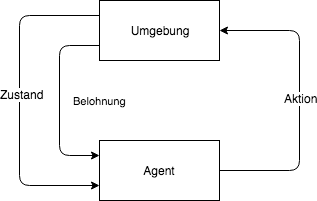
\includegraphics[width=8cm]{reinforcement-learning.png}
	\caption{Lernen durch Verstärkung}
	\label{fig:reinforcement-learning}
\end{figure}

Der Zustand $s_t \in S$ beschreibt die Umgebung des Roboters und ihn selbst zu einem bestimmten Zeitpunkt. Dies geschieht mit einer gewissen Abstraktion, da die Re\-a\-li\-tät meist zu komplex ist um diese genau abzubilden und dem Agenten durch Mess\-un\-ge\-nau\-ig\-keiten oder Ähnliches die Informationen fehlen. Aus dem vorliegenden Zustand wird die passende Aktion $a_t \in A$ durch eine Strategie, $\pi: S \rightarrow A$, ausgewählt. Diese wird anschließend ausgeführt und die von der Umgebung zurückgelieferte Reaktion bzw. reward untersucht. Durch diesen wird die Strategie optimiert. \cite{Ertel_2013}\par
Die Strategie $\pi$ ist optimal, wenn langfristig ein maximaler Ertrag erreicht wird. Der Wert bzw. die Belohnung der  optimale Strategie wird durch die Bewertungsfunktion 
\begin{equation}
	\label{value_function_max}
	V^{\pi}(s_t) = \sum_{i=0}^{\infty}\gamma^{i}r_{t+1}
\end{equation}
beschrieben, in der die direkten Belohnungen durch den Faktor $0 < \gamma < 1$ stärker einfließen, als weiter in der Zukunft liegende. Durch dieses kann der Agent in jedem Zustand die optimale Aktion auswählen. \cite{Ertel_2013}\par
Dies führt in der Robotik zu Problemen, da meist nicht klar ist, was für ein Zustand nach der Ausführung einer Aktion angenommen wird. Da der Wert der Strategie auf die Bewertung der Nachfolgezustände basiert, kann dies nicht angewendet werden. Als Lösung hat sich das Verfahren Q-Learning etabliert, dass durch Umstellung der Gleichung \ref{value_function_max} ereicht werden kann.

\section{Q-Learning} % (fold)
\label{sec:q_learning}

Beim Q-Learning wird die Bewertungsfunktion $Q(s_t, a_t)$ eingeführt. Die optimale Aktion zu einem gegebenen Zustand wird nun durch die maximale Bewertungsfunktion für den Zustand definiert. Durch Umformung der Gleichung \ref{value_function_max} wird der Wert der optimalen Bewertungsfunktion mit
\begin{equation}
	Q^{*}_t = r_t + \gamma Q^{*}_{t+1}
\end{equation} 
definiert. Der Wert der aktuellen Bewertungsfunktion ist somit die Belohnung des aktuellen Zustandes und der Wert der abgeschwächten Nachfolgezustandsbewertungsfunktion. Des Weiteren benutzt man meist noch eine Lernrate $\alpha$:
\begin{equation}
	Q(s_t, a_t) = Q(s_t, a_t) + \alpha[r_t + \gamma \ max_a Q(s_{t+1}, a_{t+1}) - Q(s_t, a_t)]
\end{equation}
Durch $\epsilon$ wird mit einer gewissen Wahrscheinlichkeit nicht die optimale, sondern eine zufällige Aktion, ausgeführt. \cite{Ertel_2013}\par
Zu Anfang werden die Werte der Bewertungsfunktionen zufällig initialisiert. Für den aktuellen Zustand wird die Aktion mit der größten Bewertungsfunktion ausgeführt, der neue Zustand und die daraus resultierende Belohnung analysiert. Der Wert der Bewertungsfunktion $Q(a, b)$ wird aktualisiert. Anschließend wird mit dem neuen Zustand wie mit dem Vorherigen verfahren. Dies wiederholt sich bis ein Endzustand erreicht worden ist. \cite{Ertel_2013}\par
Der Einsatz von Q-Learning für einen Linienfolger wird im nächsten Kapitel anhand zweier verschiedener Linienfolger evaluiert.
% section q_learning (end) % Externe Datei einbinden
\chapter{Implementierung} % (fold)
\label{cha:implementierung}



% chapter implementierung (end) % Externe Datei einbinden
\chapter{Evaluation} % (fold)
\label{cha:evaluation}

Für die Erprobung des Q-Learning-Algorithmus wurden zwei Linienfolger und eine Teststrecke konzipiert und aufgebaut. Der Kurs (siehe Abbildung \ref{fig:kurs}) besteht aus verschiedenen Geraden- und Kurvenstücken von variablem Schwierigkeitsgrad.

\begin{figure}[!htb]
	\centering
	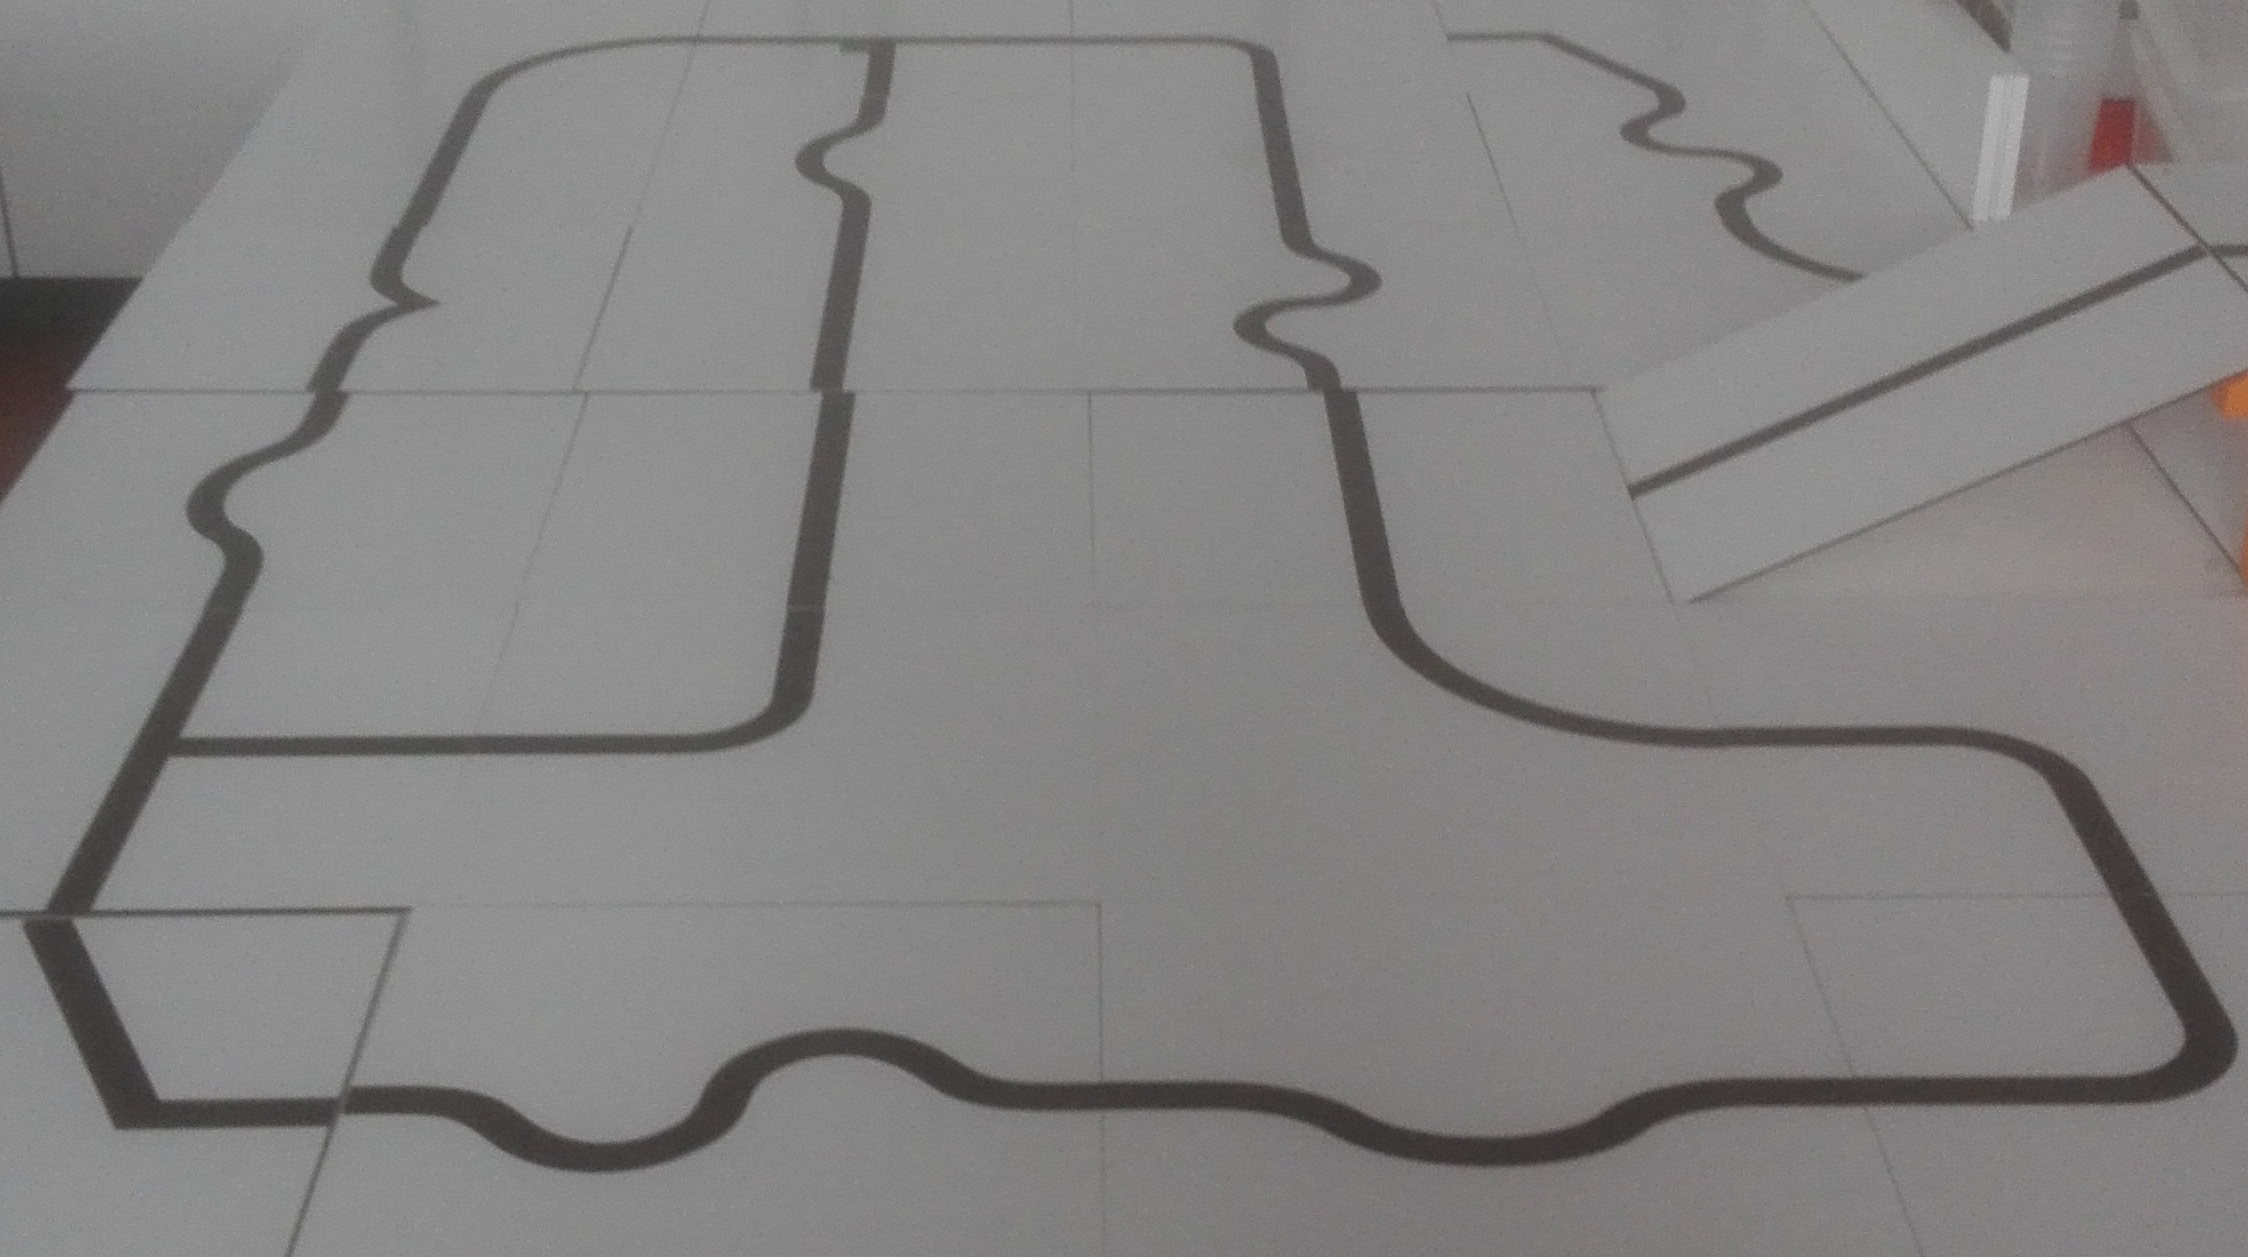
\includegraphics[width=8cm]{kurs.png}
	\caption{Kurs}
	\label{fig:kurs}
\end{figure}

Die beiden Linienfolger unterscheiden sich in der Anzahl und der Anordnung der Farbsensoren. Der erste Linienfolger $L_0$ verfügt über drei Farbsensoren (siehe Abbildung \ref{fig:linienfolger-drei-sensoren}), die nebeneinander angeordnet sind. Die schwarze Linie besitzt dieselbe Breite wie der Lichtkegel eines Farbsensors. Es ist gewünscht, dass die Linie immer unter dem mittleren Sensor ist. Im Gegensatz zum ersten Linienfolger besitzt der zweite Linienfolger $L_1$ zwei Farbsensoren, die angewinkelt angeordnet sind (siehe Abbildung \ref{fig:linienfolger-zwei-sensoren}). Im optimalen Fall liegt die Linie genau in den sich überschneidenden Lichtkegeln der zwei Sensoren.

\begin{figure}[H]
    \centering
    \begin{minipage}{0.45\textwidth}
        \centering
        \includegraphics[width=0.9\textwidth]{linienfolger-drei-sensoren.png}
        \caption{$L_0$}
        \label{fig:linienfolger-drei-sensoren}
    \end{minipage}\hfill
    \begin{minipage}{0.45\textwidth}
        \centering
        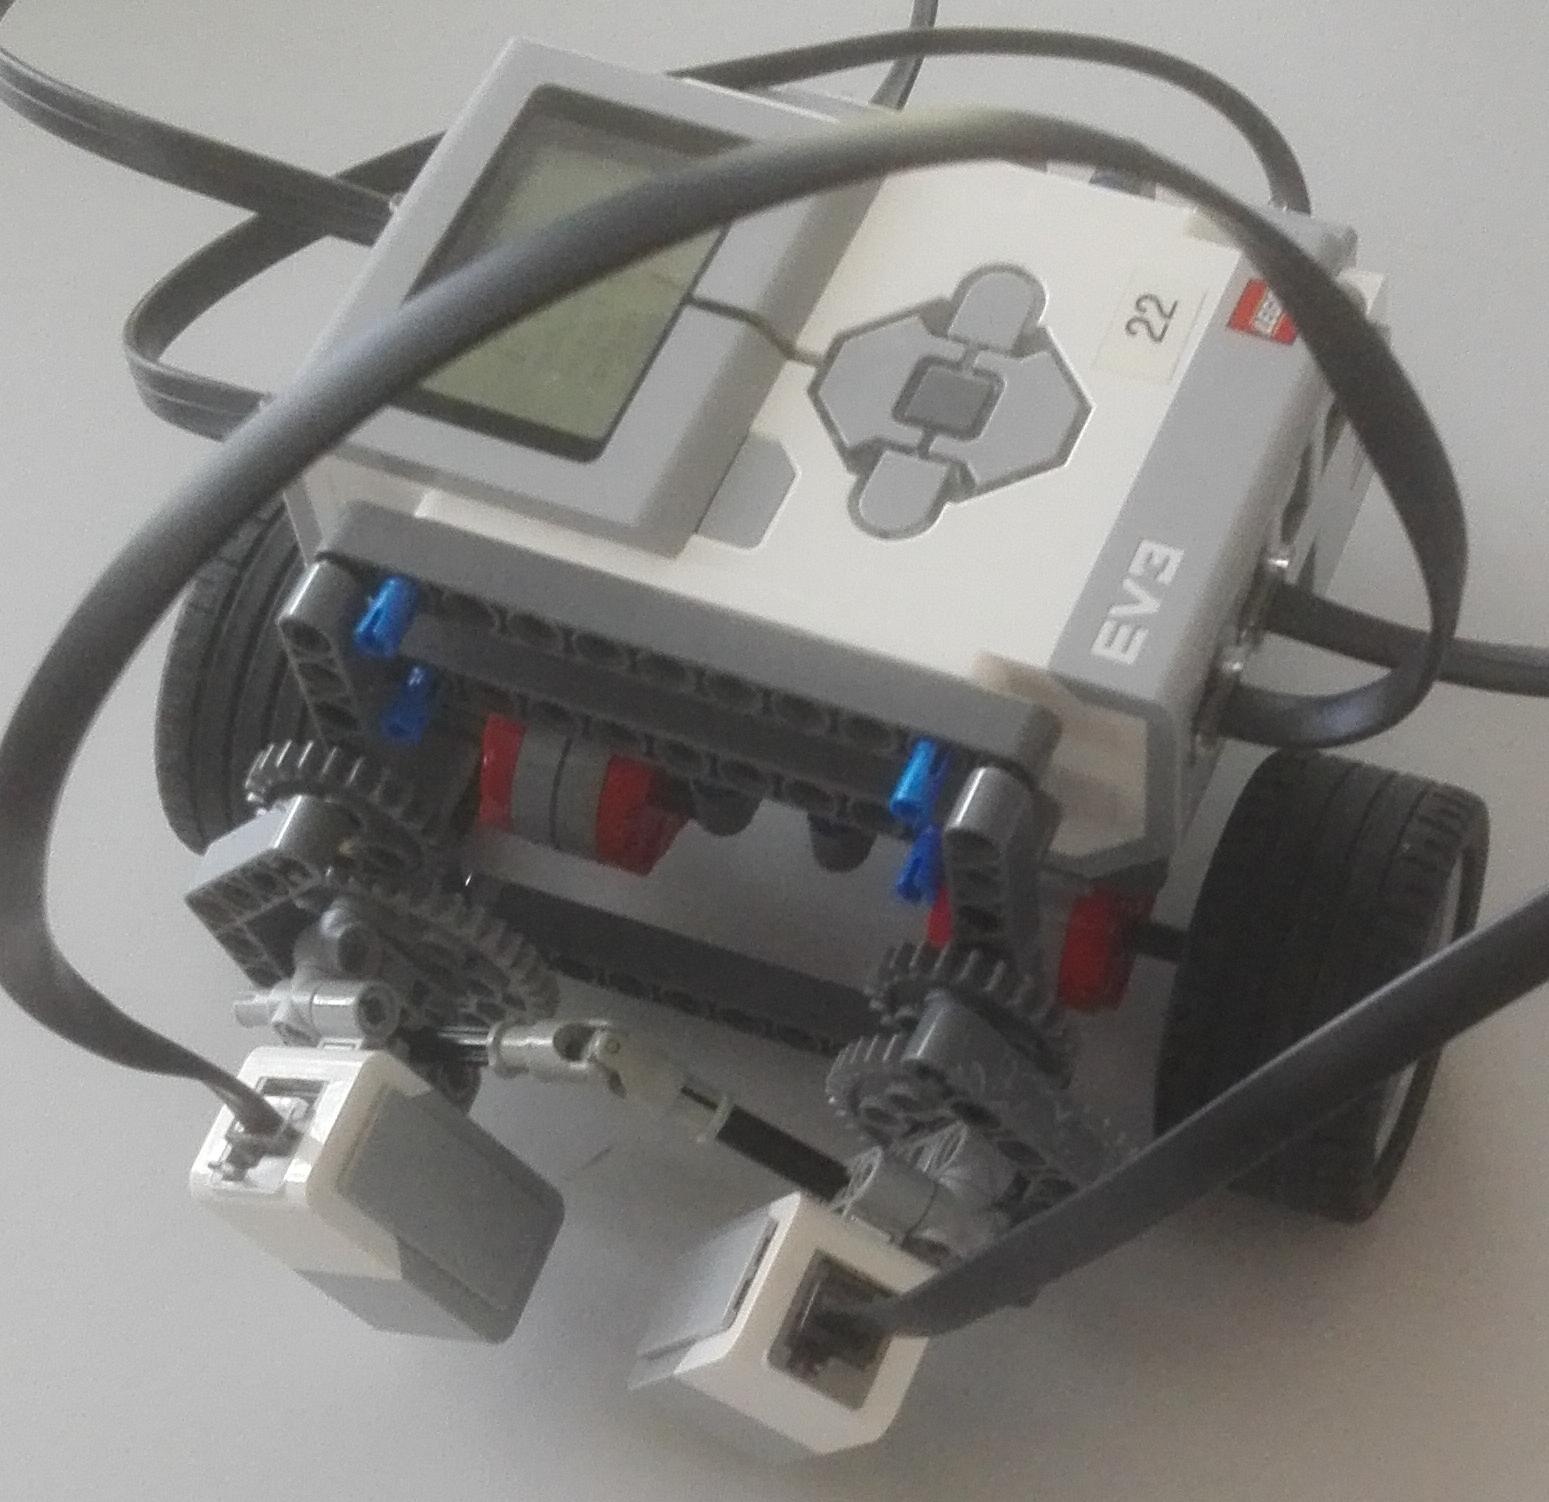
\includegraphics[width=0.9\textwidth]{linienfolger-zwei-sensoren.png}
        \caption{$L_1$}
        \label{fig:linienfolger-zwei-sensoren}
    \end{minipage}
\end{figure}

Die Sensoranordnungen der Linienfolger führt zu zwei unterschiedlichen Zustandsräumen. Die Zustände beider Linienfolger sind in den Tabellen \ref{tab:zustaende_drei_sensoren} und \ref{tab:zustaende_zwei_sensoren} angegeben.

\begin{table}[H]
  \caption{Zustandstabelle für $L_0$}
  \label{tab:zustaende_drei_sensoren}
  \renewcommand{\arraystretch}{1.2}
  \centering
  \sffamily
  \begin{footnotesize}
    \begin{tabular}{l l l}
    \toprule
    \textbf{Zustand} & \textbf{Beschreibung} & \textbf{Belohnung}\\
    \midrule
    $s_0$	&	Alle Sensoren erkennen Weiß.	&	0\\ % 000
    $s_1$	&	Der rechte Sensor erkennt Schwarz.	&	0\\ % 001
    $s_2$	&	Der mittlere Sensor erkennt Schwarz.	&	1\\ % 010
    $s_3$	&	Der mittlere und rechte Sensor erkennt Schwarz.	&	0\\ % 011
    $s_4$	&	Der linke Sensor erkennt Schwarz.	&	0\\ % 100
    $s_5$	&	Der linke und rechte Sensor erkennt Schwarz.	&	0\\ % 101
    $s_6$	&	Der linke und mittlere Sensor erkennt Schwarz.	&	0\\ % 110
    $s_7$	&	Alle Sensoren erkennen Schwarz.	&	0\\ % 111
    \bottomrule
    \end{tabular}
  \end{footnotesize}
  \rmfamily
\end{table}

\begin{table}[!htbp]
  \caption{Zustandstabelle für $L_1$}
  \label{tab:zustaende_zwei_sensoren}
  \renewcommand{\arraystretch}{1.2}
  \centering
  \sffamily
  \begin{footnotesize}
    \begin{tabular}{l l l}
    \toprule
    \textbf{Zustand} & \textbf{Beschreibung} & \textbf{Belohnung}\\
    \midrule
    $s_0$	&	Beide Sensoren erkennen Weiß.	&	0\\
    $s_1$	&	Der rechte Sensor erkennt Schwarz.	&	0\\
    $s_2$	&	Der linke Sensor erkennt Schwarz.	&	0\\
    $s_3$	&	Beide Sensoren erkennen Schwarz.	&	1\\
    \bottomrule
    \end{tabular}
  \end{footnotesize}
  \rmfamily
\end{table}

Zur Erreichung eines anderen Zustandes können beide Linienfolger folgende Aktionen (siehe Tabelle \ref{tab:aktionen}) ausführen. Beide Linienfolger benutzten die selben Motorgeschwindigkeiten und Ruhezeiten um die Vergleichbarkeit bei der Aktionsausführung zu garantieren. Beide Linienfolger nutzen für das Q-Learning die gleichen Parameter (siehe Tabelle \ref{tab:q-parameter}), um die Vergleichbarkeit der Ergebnisse zu gewährleisten.

\begin{table}
\centering

\begin{minipage}{.4\textwidth}
\caption{Aktionen}
  \label{tab:aktionen}
  \renewcommand{\arraystretch}{1.2}
  \centering
  \sffamily
  \begin{footnotesize}
    \begin{tabular}{l l}
    \toprule
    \textbf{Aktion} & \textbf{Beschreibung}\\
    \midrule
    $a_0$ & Linkskurve\\
    $a_1$ & Ge­ra­de­aus­fahrt\\
    $a_2$ & Rechtskurve\\
    \bottomrule
    \end{tabular}
  \end{footnotesize}
  \rmfamily
\end{minipage}\hfill
\begin{minipage}{.4\textwidth}
\caption{Q-Learning-Parameter}
  \label{tab:q-parameter}
  \renewcommand{\arraystretch}{1.2}
  \centering
  \sffamily
  \begin{footnotesize}
    \begin{tabular}{l l}
    \toprule
    \textbf{Parameter} & \textbf{Wert}\\
    \midrule
    $\alpha$  & $0.9$\\
    $\gamma$  & $0.2$\\
    $\epsilon$  & $0.1$\\
    \bottomrule
    \end{tabular}
  \end{footnotesize}
  \rmfamily
\end{minipage}\hfill

\end{table}

Durch theoretische Überlegungen kommt man für beide Linienfolger auf optimale Aktionen, die für einen Zustand ausgeführt werden sollen. Während diese bei $L_1$ (siehe Abbildung \ref{fig:zwei_sensoren_optimale_strategie}) leicht herzuleiten sind, ist dies bei $L_0$ (siehe Abbildung \ref{fig:drei_sensoren_optimale_strategie}) durch den größeren Zustandsraum ungleich schwieriger.\footnote{Bei beiden Graphen wurden nicht alle möglichen sinvollen Aktionen angegeben.} Bei drei Sensoren liegen zwei Zustände $s_5$ und $s_7$ vor, die nicht optimal sind. $s_5$ kann nur angenommen werden, falls $L_0$ genau auf einer Linienlücke steht.

\begin{figure}[H]
    \centering
    \begin{minipage}{0.45\textwidth}
        \centering
        \begin{tikzpicture}[->,>=stealth',shorten >=1pt,auto,node distance=2cm,
                    thick,main node/.style={circle,draw,font=\sffamily\Large\bfseries}]

          \node[main node] (1) {$s_1$};
          \node[main node] (2) [below left of=1] {$s_0$};
          \node[main node] (3) [below right of=2] {$s_3$};
          \node[main node] (4) [below right of=1] {$s_2$};

          \path[every node/.style={font=\sffamily\small}]
            (1) edge node [left] {$a_0$} (3)
            (2) edge node [left] {$a_2$} (1)
                edge [bend below] node [top] {$a_1$} (4)
            (3) edge [loop below] node {$a_1$} (3)
            (4) edge node [left] {$a_2$} (3);
        \end{tikzpicture}
        \caption{Optimale Strategie bei zwei Sensoren}
        \label{fig:zwei_sensoren_optimale_strategie}
    \end{minipage}\hfill
    \begin{minipage}{0.45\textwidth}
        \centering
        \begin{tikzpicture}[->,>=stealth',shorten >=1pt,auto,node distance=2cm,
                    thick,main node/.style={circle,draw,font=\sffamily\Large\bfseries}]

          \node[main node] (1) {$s_2$};
          \node[main node] (2) [below left of=1] {$s_1$};
          \node[main node] (3) [below right of=1] {$s_3$};
          \node[main node] (4) [below left of=2] {$s_0$};
          \node[main node] (5) [below right of=3] {$s_4$};
          \node[main node] (6) [below right of=4] {$s_7$};
          \node[main node] (7) [below left of=5] {$s_5$};
          \node[main node] (8) [below right of=6] {$s_6$};


          \path[every node/.style={font=\sffamily\small}]
            (1) edge [loop above] node {$a_1$} (1)
            (2) edge node [above] {$a_2$} (3)
                edge [loop left] node {$a_2$} (2)
            (3) edge node [right] {$a_2$} (1)
            (4) edge node [left] {$a_2$} (2)
                edge [bend above] node [above] {$a_0$} (5)
            (5) edge [bend left] node {$a_0$} (8)
                edge [bend right] node [right] {$a_0$} (1)
            (6) edge node [left] {$a_0$} (8)
                edge [bend left] node [left] {$a_2$} (3)
            (7) edge node [left] {$a_0$} (5)
                edge [bend left] node [left] {$a_2$} (2)
            (8) edge [bend right] node [left below] {$a_0$} (1);
        \end{tikzpicture}
        \caption{Optimale Strategie bei drei Sensoren} 
        \label{fig:drei_sensoren_optimale_strategie}
    \end{minipage}
\end{figure}

Bei beiden Linienfolgern wurden die optimalen Aktionen für jeden Zustand alle 200 Lernschritte archiviert (siehe Tabelle \ref{tab:q-values-three-sensors} für $L_0$ und \ref{tab:q-values-two-sensors} für $L_1$). Ein Vergleich mit den theoretisch optimalen Werten zeigt eine Abweichung. Des Weitern fluktuieren die Aktionen auch nach 2000 Lernschritten für beide Linenfolger noch beträchtlich.

\begin{table}[h]
  \caption{Q-Werte für zwei Sensoren}
  \label{tab:q-values-two-sensors}
  \renewcommand{\arraystretch}{1.2}
  \centering
  \sffamily
  \begin{footnotesize}
    \begin{tabular}{l l l l l l l l l}
    \toprule
    \textbf{Schritte} & \textbf{$s_0$} & \textbf{$s_1$} & \textbf{$s_2$} & \textbf{$s_3$}\\
    \midrule
    200     &       $a_2$   &       $a_1$   &       $a_1$   &       $a_0$\\
    400  &       $a_0$   &       $a_0$   &       $a_0$   &       $a_1$\\
    600  &       $a_0$   &       $a_0$   &       $a_2$       &       $a_1$\\
    800  &       $a_0$   &       $a_2$   &       $a_1$   &       $a_1$\\
    1000 &       $a_1$   &       $a_2$   &       $a_0$   &       $a_2$\\
    1200 &       $a_1$   &  $a_1$    &       $a_1$   &       $a_0$\\
    1400 &       $a_0$   &       $a_1$   &       $a_0$   &       $a_0$\\
    1600 &       $a_2$   &       $a_0$   &       $a_0$   &       $a_2$\\
    1800 &  $a_2$    &       $a_2$   &       $a_1$   &       $a_2$\\
    2000 &       $a_2$   &       $a_2$   &       $a_0$   &       $a_0$\\
    \bottomrule
    \end{tabular}
  \end{footnotesize}
  \rmfamily
\end{table}

\begin{table}[h]
  \caption{Q-Werte für drei Sensoren}
  \label{tab:q-values-three-sensors}
  \renewcommand{\arraystretch}{1.2}
  \centering
  \sffamily
  \begin{footnotesize}
    \begin{tabular}{l l l l l l l l l}
    \toprule
    \textbf{Schritte} & \textbf{$s_0$} & \textbf{$s_1$} & \textbf{$s_2$} & \textbf{$s_3$} & \textbf{$s_4$} & \textbf{$s_5$} & \textbf{$s_6$} & \textbf{$s_7$}\\
    \midrule
    200     &       $a_0$   &       $a_1$   &       $a_2$   &       $a_0$   &       $a_0$   &       $a_2$   &       $a_0$   &       $a_0$\\
    400  &       $a_0$   &       $a_0$   &       $a_1$   &  $a_0$    &       $a_1$   &       $a_2$   &       $a_0$   &       $a_0$\\
    600  &       $a_1$   &       $a_2$   &       $a_2$   &       $a_0$   &       $a_1$   &       $a_2$   &       $a_0$   &  $a_2$\\
    800   &       $a_0$   &       $a_2$   &       $a_2$   &       $a_1$   &       $a_1$   &       $a_2$   &       $a_0$   &       $a_2$\\
    1000 &       $a_2$   &       $a_0$   &       $a_2$       &       $a_1$   &       $a_1$   &       $a_1$   &       $a_2$   &       $a_2$\\
    1200 &       $a_2$   &       $a_0$   &       $a_2$   &       $a_2$   &       $a_2$   &       $a_1$   &  $a_2$    &       $a_1$\\
    1400 &       $a_2$   &       $a_2$   &       $a_0$   &       $a_2$   &       $a_0$   &       $a_0$   &       $a_2$   &       $a_0$\\
    1600 &       $a_1$   &       $a_2$       &       $a_0$   &       $a_2$   &       $a_0$   &       $a_0$   &       $a_2$   &       $a_0$\\
    1800 &       $a_1$   &       $a_2$   &       $a_2$   &       $a_2$   &       $a_0$   &  $a_0$    &       $a_2$   &       $a_0$\\
    2000 &       $a_1$   &       $a_2$   &       $a_0$   &       $a_2$   &       $a_1$   &       $a_0$   &       $a_2$   &       $a_0$\\
    \bottomrule
    \end{tabular}
  \end{footnotesize}
  \rmfamily
\end{table}

Der Einsatz von drei Sensoren in $L_0$ führt zu neuen Schwierigkeiten, da für manche Zustände die optimale Lösung von der auftretenden Situation abhänig ist und somit eine einmal gelerente Lösung zu einem späteren Zeitpunkt zu einer faschen Lösung führen kann.\par
Bei $L_1$ ist die gewinkelte Anordnung der Sensoren ein Problem, da die Lichtkegel der Sensoren sich nicht hundertprozentig überschneiden. Die beiden Lichtkegel überschneiden sich nur in den Außenbereichen. Dies läst sich aufgrund der vor\-ge\-ge\-benen Legobauteile nicht vermeiden. Dies führt zu einer fehlerhaften Erkennung von $s_3$. Des Weiteren können die Sensoren aufgrund der Bauweise nicht star befestigt werden und schwanken somit im Bereich der Lichtkegel. Dies führt zu Messungenauigkeiten. Bei drei Sensoren kann der Linienfolger zwischen den Zuständen $s_1$ und $s_4$ wechseln, ohne vom Fleck zu kommen. Dies kann durch Herabsetzung der Ruhezeiten oder der Motorgeschwindigkeit behoben werden.\par
Im Allgemeinen ist die optimale Kombination aus Ruhezeiten und Motorgeschwindigkeit von der Sensoranzahl und -anordnung abhängig. Diese ist bei beiden Linienfolgern noch nicht optimal. 

% chapter evaluation (end) % Externe Datei einbinden
\chapter{Fazit} % (fold)
\label{cha:fazit}

Fazit

% chapter fazit (end) % Externe Datei einbinden
% ------------------------------------------------------------------

\label{lastpage}

% Neue Seite
\cleardoublepage

% Backmatter mit normalem Zeilenabstand setzen
\singlespacing

% Römische Ziffern für die "Back-Matter", fortlaufend mit "Front-Matter"
\pagenumbering{roman}
\setcounter{page}{\value{frontmatterpage}}

% Abkürzungsverzeichnis
\addchap{\hsmaabbreviations}
% Die längste Abkürzung kann in die eckigen Klammern
% bei \begin{acronym} geschrieben, um einen häßlichen
% Umbruch zu verhindern
\begin{acronym}[IEEE]
\acro{ABK}{Abkürzung}
\acro{ACM}{Association of Computing Machinery}
\acro{PDF}{Portable Document Format}
\acro{IEEE}{Institute of Electrical and Electronics Engineers}
\acro{ISO}{International Organization for Standardization}
\end{acronym}


% Tabellenverzeichnis erzeugen
%\cleardoublepage
\phantomsection
\addcontentsline{toc}{chapter}{\hsmalistoftables}
\listoftables

% Abbildungsverzeichnis erzeugen
%\cleardoublepage
\phantomsection
\addcontentsline{toc}{chapter}{\hsmalistoffigures}
\listoffigures

% Listingverzeichnis erzeugen
%\cleardoublepage
\phantomsection
\addcontentsline{toc}{chapter}{\hsmalistings}
\lstlistoflistings

% Literaturverzeichnis erzeugen
\begin{flushleft}
\printbibliography
\end{flushleft}

% Index ausgeben. Wenn Sie keinen Index haben, entfernen Sie einfach
% diesen Teil.
%\cleardoublepage
%\phantomsection
%\addcontentsline{toc}{chapter}{\hsmaindex}
%\printindex

% Anhang. Wenn Sie keinen Anhang haben, entfernen Sie einfach
% diesen Teil.
%\appendix
%\chapter{Erster Anhang}

Hier ein Beispiel für einen Anhang. Der Anhang kann genauso in Kapitel und Unterkapitel unterteilt werden, wie die anderen Teile der Arbeit auch.

%\chapter{Zweiter Anhang}

Hier noch ein Beispiel für einen Anhang.


\end{document}
